\section{Reference Time Cuts} \label{sec:reftime}

Figure~\ref{fig:reference_time_cartoon} illustrates the relationship
between a detector signal and the internal clocks of the CAEN 1190 TDCs that
determine the timing resolution of measurements in Hall C.
An L1 pretrigger (see Section~\ref{sec:daq}) that initiates read-out
in a ROC latches onto the leading edge of the next cycle of an 1190's
\SI{40}{\mega\hertz} clock.
As a result, this digitized pretrigger time can only be known to have been
received within the \SI{25}{\nano\second} window between that
\SI{40}{\mega\hertz} cycle and the previous cycle.
Pretriggers also have an intrinsic \SI{4}{\nano\second}
jitter\footnote{A small, irregular variation in an otherwise periodic signal.},
meaning that raw TDC signals can only be known to within
\SI{\sim29}{\nano\second}.
To improve the timing resolution, the DAQ sends a delayed copy of the
pretrigger, called a \textit{reference time}, to the TDC.
The reference time latches onto the leading edge of the 1190's
\SI{10}{\giga\hertz} clock (accurate to \SI{0.1}{\nano\second}), and initiates
read-out of the full TDC spectrum (a lookback window of a few
\si{\micro\second}).
All modules in a given ROC share the same reference time.
Therefore, subtracting the raw TDC time (synced to the \SI{40}{\mega\hertz}
clock) from the reference time (synced to the \SI{10}{\giga\hertz} clock),
the timing resolution can be improved to approximately \SI{0.1}{\nano\second}.
This reference time subtraction is performed offline during \textit{hcana}
replay.


\begin{figure}[!h]
    \centering
    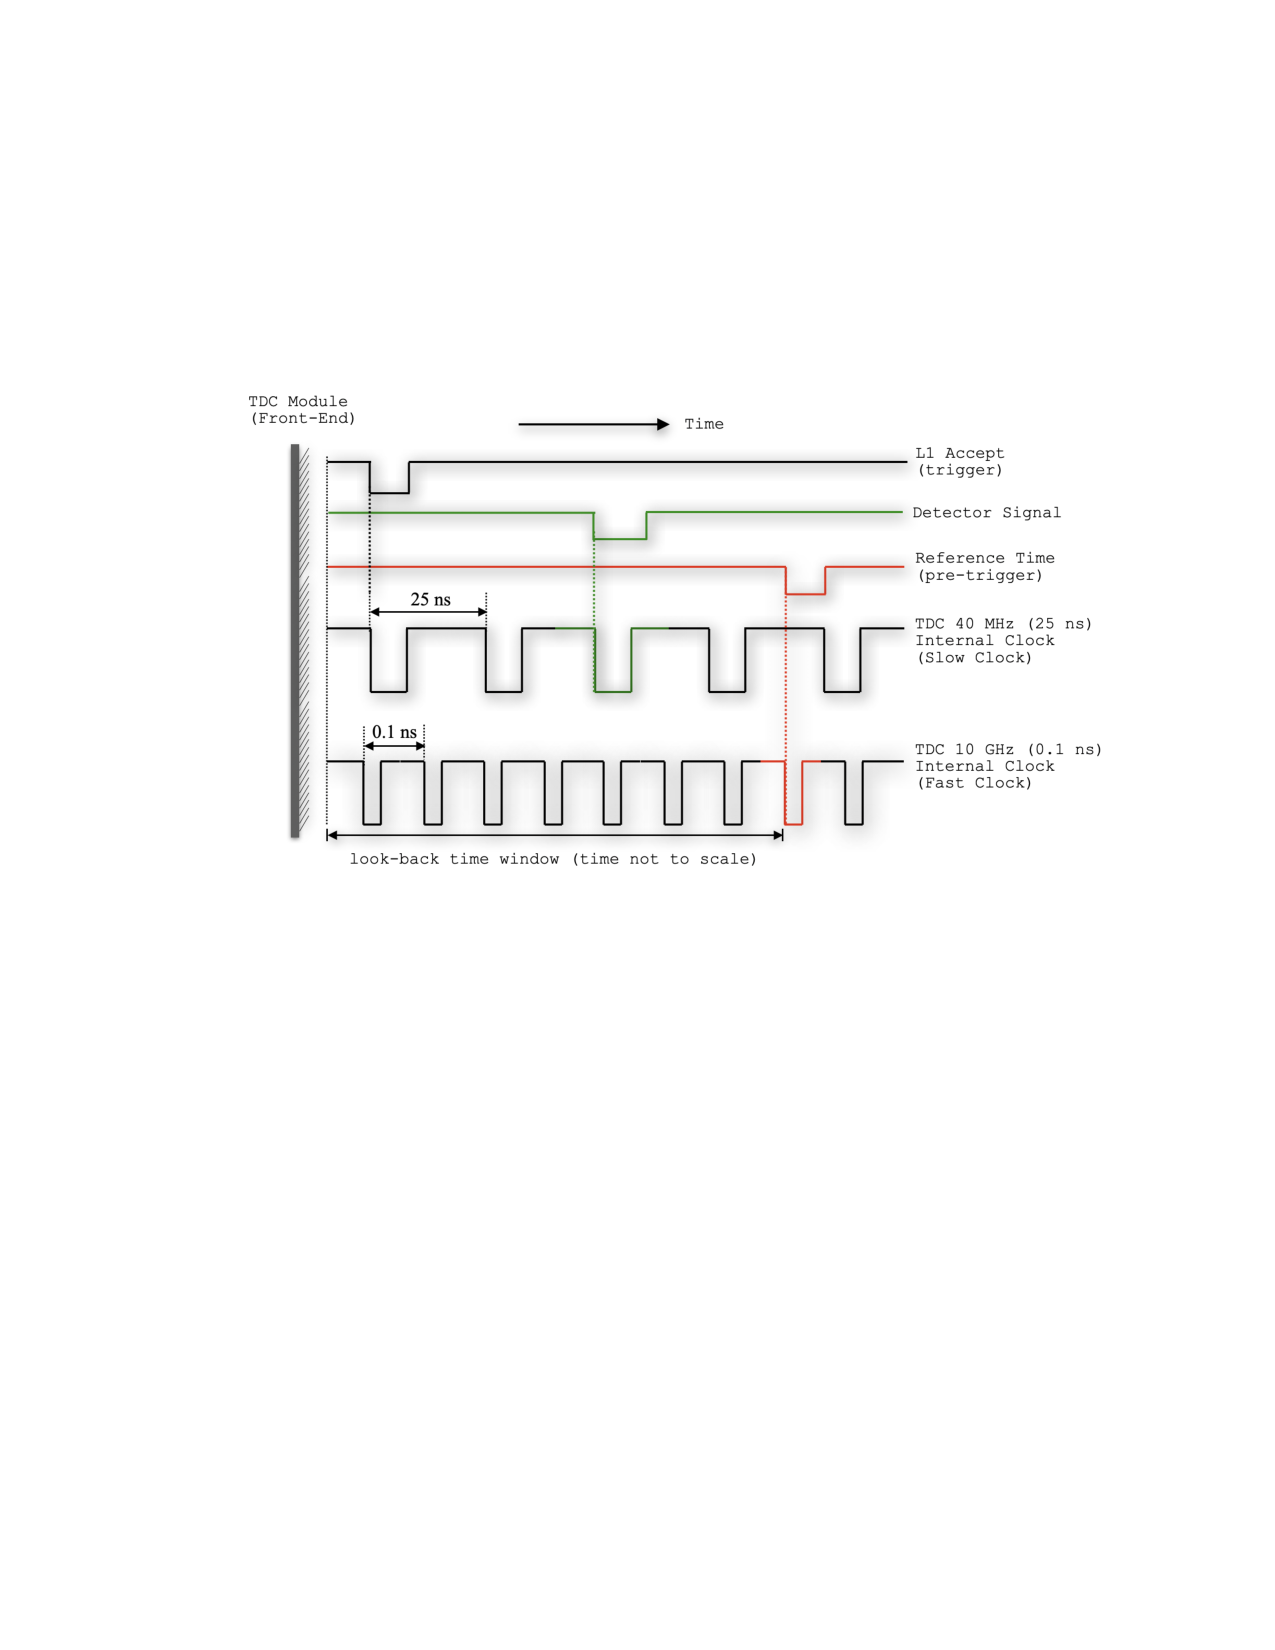
\includegraphics[width=1.0\textwidth]{chap4/yero_reftime.pdf}
    \caption{
            A cartoon illustrating the synchronization of a detector signal
            with a CAEN 1190 TDC's internal \SI{4}{\mega\hertz} and
            \SI{10}{\giga\hertz} clocks. Figure reproduced from Carlos Yero's
            PhD thesis~\cite{Yero_2020}.
            }
    \label{fig:reference_time_cartoon}
\end{figure}


% TODO: ref time cut example figure
As shown in Figure,
true physics events will lie within a range of X raw TDC channels.
Background events will have occurred earlier in the lookback window, and must
be prevented from being chosen as the reference time.
To accomplish this, \textit{hcana} uses reference time cuts defined in
the parameter files.


\section{Detector Time Window Cuts}
As with reference time selection, care must be taken to avoid background hits
in the fADC spectra.
The distribution of the differences between the fADC pulse times and
reference-time-subtracted TDC times for a given PMT in a detector should
be a narrow peak with a width determined by the resolutions of the TDCs
and fADCs.
Events far from this peak have TDC and fADC times that are not correlated, and
can be assumed not to be associated with the current event.
By placing lower and upper bounds on the difference between these times on a
per-PMT basis, we can ensure that \textit{hcana} will choose the correct fADC
hits for every event.
Example histograms of these time differences are shown in Figure
% TODO: fADC-TDC time difference example figure


\section{Livetime} \label{sec:livetime}
When a trigger is accepted, the DAQ system is unable to accept additional
triggers for a time determined by the gate widths of front end electronics and
the time it takes for CODA to write the event to disk.
The time during which the DAQ is unable to accept another event is referred to
as deadtime.
The inverse concept, livetime, refers to the total time that the DAQ is
\textit{not} occupied by processing incoming triggers.
The total livetime $TLT$ is a correction applied to the charge normalized yield
to account for events that are missed because of this phenomenon.


% TODO: edtm logic diagram
The EDTM (see Section~\ref{sec:edtm}) pulser allows an estimate of the total
livetime in a given run.
It sends regular pulses at a low frequency (\SI{3}{\hertz} in our experiment) at the
trigger logic level in the counting house.
By comparing the number of triggers that are accepted by the DAQ to the number
of pulses that are counted by the EDTM scaler, we can estimate the total
livetime as
\begin{equation}
    TLT = \frac{N_{EDTM,accepted}}{N_{EDTM,scaler}}
\end{equation}
where $N_{EDTM,accepted}$ is the number of events with a non-zero hit in the
EDTM TDC spectrum and $N_{EDTM,scaler}$ is the total number of EDTM triggers
counted by the EDTM scaler.
% TODO: Peter Bosted's correction. I don't understand his derivation.
% Let n be accepted, N be scaler count. Then L=n/N
% Let j be the current, and jc be the "cut current"
% Let f=j/jc
% Then Peter's correction is Lnew = (L-(1-f))/f
% The assumption here is that livetime is 100% when the beam is "off"
% i.e. below the cut value (typically a couple uA) used by hcana


% TODO: trigger rate figure
Because livetime should be dependent on trigger rate and the trigger rates
vary between our kinematic settings, we calculate a per-run livetime to
correct each run's yield.
Moreover, the EDTM system was not functional when we took our first set of data
for $Q^2$ of \SI{8}{\giga\electronvolt\squared}.
To estimate the livetime for these data, we performed a linear fit of the other
kinematics' $TLT$ dependence on SHMS 3/4 trigger rate and used this fit to
estimate the livetime for the $Q^2$=\SI{8}{\giga\electronvolt\squared} runs.

% TODO: LTE vs pTRIG1 (SHMS 3/4)

The computer livetime can be estimated as
\begin{equation}
    TLT = \frac{N_{phys,accepted}-N_{EDTM,accepted}}{N_{phys,scaler}-N_{EDTM,scaler}}
\end{equation}
The computer livetime for our data is neglible because CODA was configured to
only take coincidence events, whose rates were all quite low (below
\SI{6}{\hertz}) for all our kinematics.

% TODO: computer livetime vs pTRIG6

% TODO: add refs for Eric and Dave's slides

